%----------------------------------------------------------------------------------------
% SECTION 2
%----------------------------------------------------------------------------------------
\label{test_data}
\section{Test Data}

There are a few sources for test-data of XPS-spectra. A main database was found on XPSlibrary, provided by TXL. Further, the XPSSurfA on CMSS Hub from the Australian University La Trobe contains more than 1700 spectra of which >100 survey spectra were used for the evaluation of the model.


\subsection{Data preprocessing}

As is typical for data acquired from laboratories, XPS data comes in various formats and measurement parameters. Apart from XPS-specific parameters, the resolution and the range mostly influence the evaluation of spectra with the deep-learning framework. Thus, an automated workflow for the spectra pre-processing is introduced to provide a valid entry point to the model.
Although most wide-survey spectra are measured with a comparable energy-range, it should be identical to the training data for prediction. Thus, any signal outside the specified binding energy range (0-1000 eV) is cut off and the discrete measurement points inside the range are interpolated or subsampled by using a uniformly distributed sampling method to match 1024 points.

\begin{figure}
    \centering
    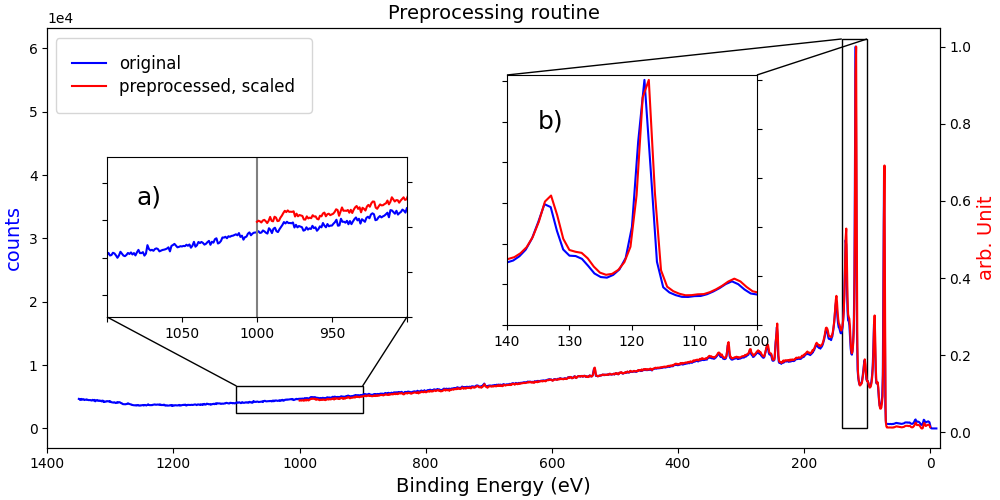
\includegraphics[width=\textwidth]{Figures/preprocessing_routine.png}
    \caption{Preprocessing routine of experimental spectra}
    \label{fig:preproc_routine}
\end{figure}

The preprocessing results of a selection of experimental spectra were then assessed, as shown in \ref{fig:ex_vs_sim}.

\begin{figure}
    \centering
    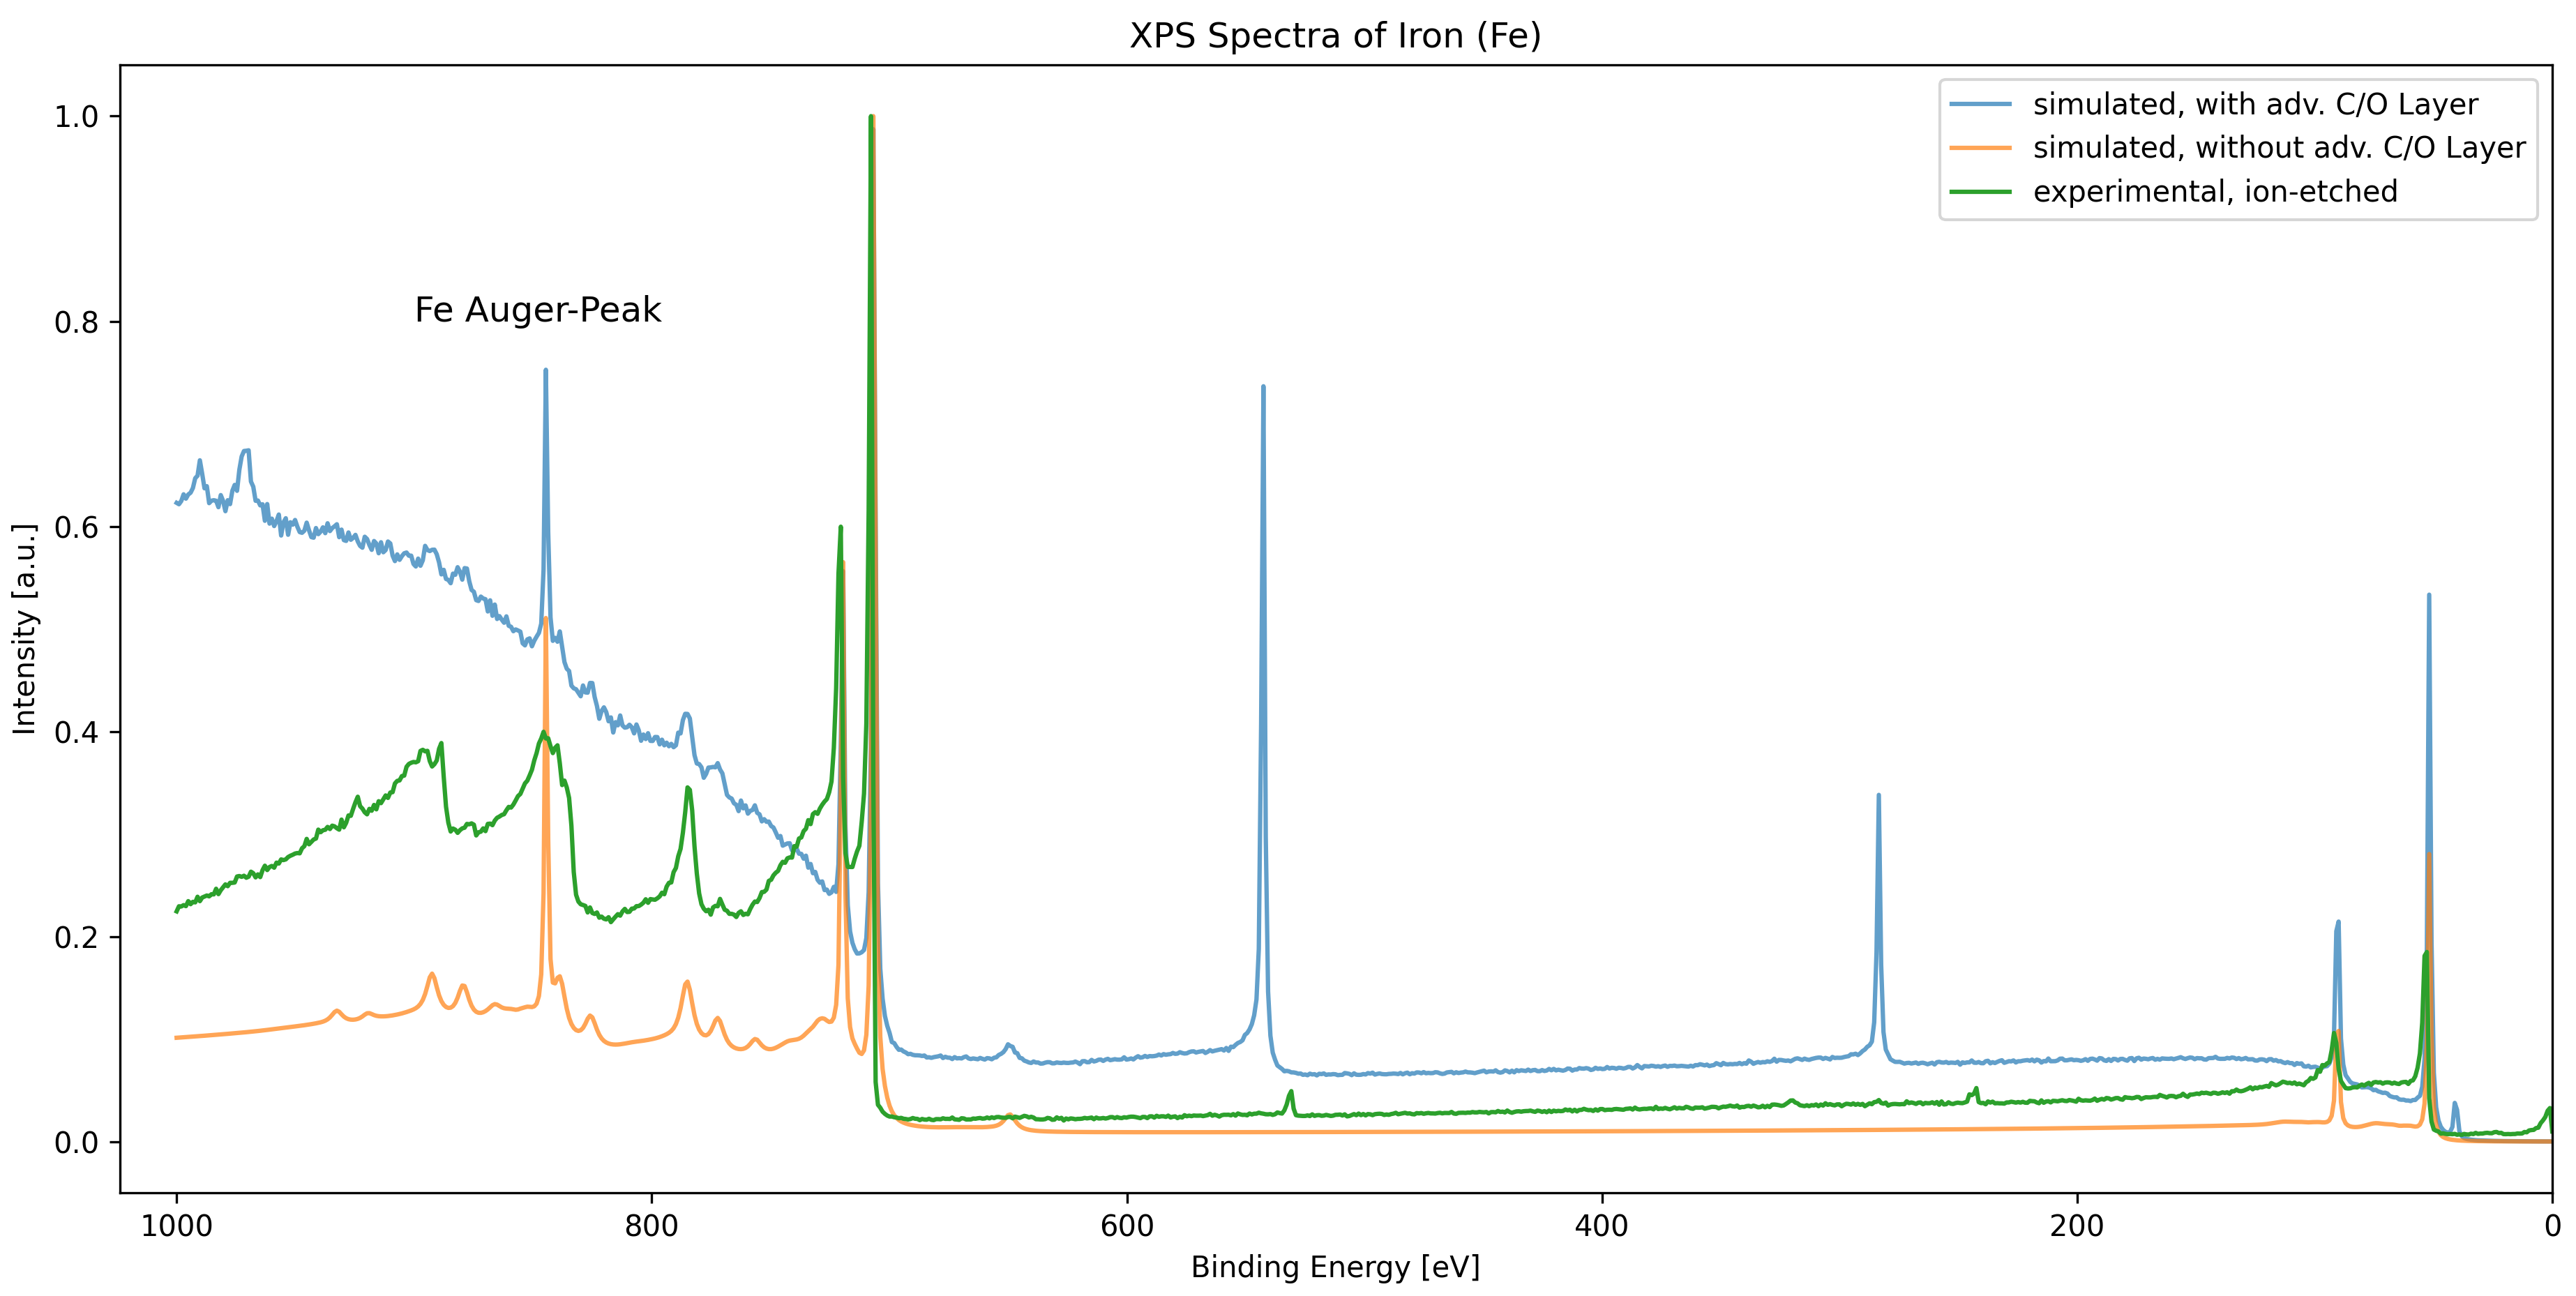
\includegraphics[width=\textwidth]{Figures/Fe_XPS.png}
    \caption{Experimental preprocessed spectrum vs. Simulated spectrum of elemental Iron}
    \label{fig:ex_vs_sim}
\end{figure}

The python module used to preprocess the data can be found in \ref{AppendixA}.